% Created 2020-04-15 mié 17:46
% Intended LaTeX compiler: pdflatex
\documentclass[presentation,aspectratio=1610]{beamer}
\usepackage[utf8]{inputenc}
\usepackage[T1]{fontenc}
\usepackage{graphicx}
\usepackage{grffile}
\usepackage{longtable}
\usepackage{wrapfig}
\usepackage{rotating}
\usepackage[normalem]{ulem}
\usepackage{amsmath}
\usepackage{textcomp}
\usepackage{amssymb}
\usepackage{capt-of}
\usepackage{hyperref}
\usepackage{khpreamble}
\usepackage{pgfplots}
\usepackage{pdfpages}
\usepackage{circuitikz}
\usepgfplotslibrary{groupplots}
\usetikzlibrary{positioning}
\renewcommand*{\not}[1]{\ensuremath{\bar{#1}}}
\renewcommand*{\not}[1]{\ensuremath{\overline{#1}}}
\usetheme{default}
\author{Kjartan Halvorsen}
\date{\today}
\title{Boolean algebra, logic diagrams and truth tables}
\hypersetup{
 pdfauthor={Kjartan Halvorsen},
 pdftitle={Boolean algebra, logic diagrams and truth tables},
 pdfkeywords={},
 pdfsubject={},
 pdfcreator={Emacs 26.3 (Org mode 9.3.6)}, 
 pdflang={English}}
\begin{document}

\maketitle

\section{Boolean algebra, minterms and maxterms}
\label{sec:org605a59f}
\begin{frame}[label={sec:orgb501097}]{AND and OR}
\(a, b \in \{0,1\}\)
\begin{columns}
\begin{column}{0.5\columnwidth}
\begin{block}{AND}
\begin{center}
\begin{tabular}{|cc|c|}
\hline
\(a\) & \(b\) & \(a\) AND \(b\), \(ab\)\\
\hline
0 & 0 & 0\\
0 & 1 & 0\\
1 & 0 & 0\\
1 & 1 & 1\\
\hline
\end{tabular}
\end{center}

\begin{center}
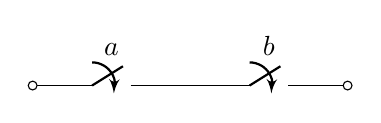
\begin{tikzpicture}
  \draw (0,0) to[switch, label=$a$, o-] (2,0) to[switch, label=$b$, -o] (4, 0);
\end{tikzpicture}
\end{center}
\alert{Closed circuit \(\Leftrightarrow\) 1}

\alert{Open circuit \(\Leftrightarrow\) 0}

\begin{center}
\includegraphics[width=0.5\linewidth]{../../figures/and-gate.pdf}
\end{center}
\end{block}
\end{column}

\begin{column}{0.5\columnwidth}
\begin{block}{OR}
\begin{center}
\begin{tabular}{|cc|c|}
\hline
\(a\) & \(b\) & \(a\) OR \(b\), \(a+b\)\\
\hline
0 & 0 & 0\\
0 & 1 & 1\\
1 & 0 & 1\\
1 & 1 & 1\\
\hline
\end{tabular}
\end{center}

\begin{center}
\begin{tikzpicture}
  \draw (0,0) to[switch, label=$a$, o-o] (4,0);
  \draw (1,0) to[short] (1,-1) to[switch, l_=$b$, ] (3, -1) to[short] (3, 0);
\end{tikzpicture}
\end{center}

\begin{center}
\includegraphics[width=0.5\linewidth]{../../figures/or-gate.pdf}
\end{center}
\end{block}
\end{column}
\end{columns}
\end{frame}


\begin{frame}[label={sec:org1573679}]{NAND and NOR}
\(a, b \in \{0,1\}\)
\begin{columns}
\begin{column}{0.5\columnwidth}
\begin{block}{NAND}
\begin{center}
\begin{tabular}{|cc|c|}
\(a\) & \(b\) & \(a\) NAND \(b\), \(\overline{a\cdot{}b}\)\\
\hline
0 & 0 & 1\\
0 & 1 & 1\\
1 & 0 & 1\\
1 & 1 & 0\\
\hline
\end{tabular}
\end{center}

\begin{center}
\includegraphics[width=0.5\linewidth]{../../figures/nand-gate.pdf}
\end{center}
\end{block}
\end{column}

\begin{column}{0.5\columnwidth}
\begin{block}{NOR}
\begin{center}
\begin{tabular}{|cc|c|}
\(a\) & \(b\) & \(a\) NOR \(b\), \(\overline{a+b}\)\\
\hline
0 & 0 & \\
0 & 1 & \\
1 & 0 & \\
1 & 1 & \\
\hline
\end{tabular}
\end{center}

\begin{center}
\includegraphics[width=0.5\linewidth]{../../figures/nor-gate.pdf}
\end{center}
\end{block}
\end{column}
\end{columns}
\end{frame}

\begin{frame}[label={sec:org2d0b9ef}]{Boolean algebra, contd}
\(x, y, z \in \{0,1\}\)

\begin{center}
\begin{tabular}{r|c|c|}
 & Property & Dual\\
\hline
Properties of 0 and 1 & \(x+0=x\) & \(x\cdot 0=0\)\\
 & \(x+1=1\) & \(x \cdot 1 = x\)\\
Idempotency & \(x+x=x\) & \(x\cdot x = x\)\\
Complementarity & \(x+\not{x}=1\) & \(x\cdot \not{x}=0\)\\
Involution & \(\not{\not{x}}=x\) & \\
Commutative & \(x+y=y+x\) & \(x\cdot y = y\cdot x\)\\
Associative & \((x+y) + z = x + (y+z)\) & \((xy)z = z(yz)\)\\
Distributive & \(x\cdot (y+z) = xy + xz\) & \(x+yz=(x+y)(x+z)\)\\
\hline
\end{tabular}
\end{center}
\end{frame}

\begin{frame}[label={sec:orge5065a4}]{Boolean algebra, contd}
\(x, y \in \{0,1\}\)

\begin{center}
\begin{tabular}{r|c|c|}
 & Theorem & Dual\\
\hline
Absorption & \(x+xy=x(1+y)=x\) & \(x(x+y)=x\)\\
Logic adjacency & \(xy + x\not{y} = x(y+\not{y}) =x\) & \((x+y)(x+\not{y}) = x\)\\
De Morgan's & \(\not{x+y}=\not{x}\cdot{}\not{y}\) & \(\not{xy} = \not{x} + \not{y}\)\\
\hline
\end{tabular}
\end{center}
\end{frame}

\begin{frame}[label={sec:orgd14be63}]{DeMorgan's theorem}
\begin{center}
\includegraphics[width=0.4\linewidth]{../../figures/Demorganlaws.png} From wikipedia
\end{center}
\end{frame}
\begin{frame}[label={sec:orgbb8fe29}]{Simplify functions}
\begin{enumerate}
\item \(f = (a+b)(a+c)\)
\item \(f = a + \not{a}b\)
\end{enumerate}
\end{frame}


\begin{frame}[label={sec:orgd9a80c9}]{Logic diagram \(\rightarrow\) function}
Determine the function represented by the logic diagrams
\begin{center}
\includegraphics[width=0.7\linewidth]{../../figures/exercise-gate-4.pdf}
\end{center}
\end{frame}


\begin{frame}[label={sec:org42b2888}]{Function \(\rightarrow\) logic diagram}
Draw the diagram corresponding to the boolean function
\begin{enumerate}
\item \(f = (a+b)(a+c)\)
\item \(f = a + \not{a}b\)
\end{enumerate}
\end{frame}


\begin{frame}[label={sec:org98e40c3}]{Group exercise}
\begin{enumerate}
\item Enter breakout room
\item One of you downloads and shares this presentation
\item Work together on the problems in the previous three slides
\begin{enumerate}
\item Simplify functions
\item Determine function from logic diagram
\item Draw logic diagram from function
\end{enumerate}
\end{enumerate}
\end{frame}
\end{document}